%!TEX TS-program = xelatex
\documentclass[]{friggeri-cv}
\usepackage{afterpage}
\usepackage{hyperref}
\usepackage{color}
\usepackage[normalem]{ulem}
\usepackage{xcolor}
\hypersetup{
    pdftitle={},
    pdfauthor={},
    pdfsubject={},
    pdfkeywords={},
    colorlinks=false,       % no lik border color
   allbordercolors=white    % white border color for all
}
\addbibresource{bibliography.bib}
\RequirePackage{xcolor}
\definecolor{pblue}{HTML}{0395DE}

\makeatletter
\let\old@rule\@rule
\def\@rule[#1]#2#3{\textcolor{rulecolor}{\old@rule[#1]{#2}{#3}}}
\makeatother

\definecolor{rulecolor}{named}{gray}

\begin{document}
\header{Vincent}{Castelluci}
      {Développeur Full stack}
\hfill \lq\textit{Do, fail, improve}\rq

\rule{397pt}{8pt}

% In the aside, each new line forces a line break
\begin{aside}
  \section{Addresse}
  \hspace{1cm}
    19 rue de Thizy
    69470, Cours-la-ville
    France
  \section{Contacts}
  \hspace{1cm}
    \vspace{0.5mm}
\includegraphics[scale=0.60]{img/france.png}~\href{tel:+33634321575}{+336 3432 1575}
    \vspace{0.5mm}\hspace{-2cm}\href{mailto:vincent.castelluci@gmail.com}{
\includegraphics[scale=0.60]{img/mail.png}~vincent@castelluci.xyz}
    \vspace{0.5mm}\href{https://www.linkedin.com/in/vincent-castelluci-363939170}{
\includegraphics[scale=0.60]{img/linkedin.png}~vincent-castelluci}
    \vspace{0.5mm}\href{skype://vincent690022?userinfo}{
\includegraphics[scale=0.60]{img/skype.png}~vincent690022}
    \vspace{0.5mm}\href{https://github.com/hypr2771}{
\includegraphics[scale=0.60]{img/github.png}~hypr2771}
    ~
  \section{Compétences}
  \hspace{1cm}
    \textbf{Learning}
\includegraphics[scale=0.40]{img/5puces.png}
    \textbf{Java}
\includegraphics[scale=0.40]{img/5puces.png}
    \textbf{TDD}
\includegraphics[scale=0.40]{img/5puces.png}
    \textbf{JavaScript}
\includegraphics[scale=0.40]{img/4puces.png}
    \textbf{Solidity}
\includegraphics[scale=0.40]{img/3puces.png}
    \textbf{HTML}
\includegraphics[scale=0.40]{img/4puces.png}
    \textbf{CSS}
\includegraphics[scale=0.40]{img/3puces.png}
    \textbf{Python}
\includegraphics[scale=0.40]{img/2puces.png}
    \textbf{Spring}
\includegraphics[scale=0.40]{img/4puces.png}
    \textbf{React}
\includegraphics[scale=0.40]{img/3puces.png}
    \textbf{Pipelines}
\includegraphics[scale=0.40]{img/5puces.png}
    \textbf{Git}
\includegraphics[scale=0.40]{img/4puces.png}
    \textbf{Maven}
\includegraphics[scale=0.40]{img/4puces.png}
    \textbf{Docker}
\includegraphics[scale=0.40]{img/3puces.png}
    \textbf{SQL}
\includegraphics[scale=0.40]{img/3puces.png}
    \textbf{GNU/Linux}
\includegraphics[scale=0.40]{img/4puces.png}
    \textbf{Windows}
\includegraphics[scale=0.40]{img/3puces.png}
    ~
  \section{Personnalité}
  \hspace{1cm}
    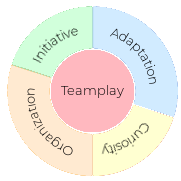
\includegraphics[scale=0.62]{img/personal.png}
    ~
  \section{Langues}
  \hspace{1cm}
    \textbf{Français}
\includegraphics[scale=0.40]{img/5puces.png}
    \textbf{Anglais}
\includegraphics[scale=0.40]{img/4puces.png}
    \textbf{Thai}
\includegraphics[scale=0.40]{img/2puces.png}
    \textbf{Allemand}
\includegraphics[scale=0.40]{img/2puces.png}
\end{aside}

\section{Résumé}
Développeur full stack expérimenté, dont les préoccupations principales sont le résultat et la qualité logicielle.\\
J'aime apprendre, appliquer et rechercher de nouvelles solutions par moi même afin d'améliorer la "Quality of Life" (cycle de vie, méthodologies, pipelines \& CI/CD...) de mes projets.\\
Mes expériences passées m'ont littéralement forgé et appris tant de choses; la plus importante est que l'unique moyen de réussir et d'essayer, échouer et \textit{s'améliorer} -- raison pour laquelle j'utilise autant que faire se peut le TDD.\\
Je suis idéallement à la recherche de missions dont les attentes de qualité et de résultats sont élevées, dans des domaines encore inexplorés ou que je connais déjà très bien, sur place ou en télétravail.\\
\textbf{Ce que je ne cherche pas :}
\begin{itemize}
\item une équipe qui refuse de comprendre la valeur du TDD
\vspace{-\baselineskip}
\vspace{1 ex}
\item une équipe où les qualités humaines sont relayées au second plan
\vspace{-\baselineskip}
\vspace{1 ex}
\item une équipe appliquant bêtement les méthodes d'un livre sans faire preuve d'intelligence
\vspace{-\baselineskip}
\vspace{-\baselineskip}
\vspace{1 ex}
\item une équipe qui stagne et ne s'améliore pas
\end{itemize}

\section{Expériences}
\begin{entrylist}
  \entry
    {07/18 - Now}
    {Développeur full stack}
    {Freelance, en télétravail ou sur place, Monde entier}
    {En cours de développement de mon projet personnel, je deviens de jours en jours plus familier avec les outils DevOps modernes tels que AWS, Kubernetes, BitBucket et son ecosystème; ainsi que les outils front modernes tels que React.js, Bulma et SASS.\\}
    \entry
    {06/16 - 07/18}
    {Lead Développeur full stack}
    {Ubik Ingénierie, pour Decathlon E-Commerce, France}
    {
Mes tâches étaient entre autres :
      \begin{itemize}
        \item améliorer la qualité du périmètre paiement au travers de code reviews, tests, diffusion de best practices, mises à jour de frameworks et d'API...
        \item former les nouveaux arrivants afin d'être operationnels ASAP en rédigeant de la documentation sur les process, et en prévoyant du pair programming et/ou mob programming
        \item rendre l'application open source (tâche pas si aisée qu'elle en a l'air, car elle force à combler de nombreuses failles)
        \item rendre l'application plus robuste et resiliente en ajoutant des stress tests, en mesurant la santé et en prévoyant le DRP en cas d'urgences
      \end{itemize}
}
    \entry
    {06/14 - 06/16}
    {Développeur full stack}
    {Ubik Ingénierie pour Decathlon E-Commerce, France}
    {Ma principale mission était de maintenir, améliorer et corriger la plateforme de paiements centralisés ainsi que de l'intégrer au sein du site européen de Decathlon.\\
En arrivant chez Decathlon, l'équipe commençait une man\oe uvre de transformation agile, et ce fut un voyage long mais intéressant, qui ne finira jamais, car l'amélioration continue reste mon leitmotiv.}
\end{entrylist}

\section{Passions}

\includegraphics[scale=0.6]{img/books.png}\hspace{2.4 em}
\includegraphics[scale=0.6]{img/team.png}\hspace{2.4 em}
\includegraphics[scale=0.6]{img/programming.png}\hspace{2.4 em}
\includegraphics[scale=0.6]{img/chess.png}\hspace{2.4 em}
\includegraphics[scale=0.6]{img/formula.png}
\phantom{}\hspace{1.9 em}Livres\hspace{3.6 em}Sports collectifs\hspace{4 em}Code\hspace{3.2 em}Jeux de stratégies\hspace{1.4 em}Mathématique

%%% This piece of code has been commented by Karol Kozioł due to biblatex errors. 
% 
%\printbibsection{article}{article in peer-reviewed journal}
%\begin{refsection}
%  \nocite{*}
%  \printbibliography[sorting=chronological, type=inproceedings, title={international peer-reviewed conferences/proceedings}, notkeyword={france}, heading=subbibliography]
%\end{refsection}
%\begin{refsection}
%  \nocite{*}
%  \printbibliography[sorting=chronological, type=inproceedings, title={local peer-reviewed conferences/proceedings}, keyword={france}, heading=subbibliography]
%\end{refsection}
%\printbibsection{misc}{other publications}
%\printbibsection{report}{research reports}

\end{document}